% --------------------------------------------------------------------------- %
%                                      _                                      %
%   ___ ___  _ __ ___  _ __   ___  ___(_)_ __   __ _                          %
%  / __/ _ \| '_ ` _ \| '_ \ / _ \/ __| | '_ \ / _` |                         %
% | (_| (_) | | | | | | |_) | (_) \__ \ | | | | (_| |                         %
%  \___\___/|_| |_| |_| .__/ \___/|___/_|_| |_|\__, |                         %
%                     |_|                      |___/                          %
%                                                                             %
%                                                   __ _ _ __ ___  __ _       %
%                                                  / _` | '__/ _ \/ _` | /\/| %
%                                                 | (_| | | |  __/ (_| ||/\/  %
%                                                  \__,_|_|  \___|\__,_|      %
%                                                                             %
% --------------------------------------------------------------------------- %
\chapter{Composing area\textasciitilde{}}{Exploring Real and Virtual Environments Through Gestural Ambisonics and Audio Augmented Reality}
\label{sec: area}
%\markboth{}{Composing area\textasciitilde{}: Exploring Real and Virtual Environments Through Gestural Ambisonics and Audio Augmented Reality}
\epigraph{\emph{}}{}

\noindent \textbf{area\textasciitilde{} Code:}        \url{https://www.github.com/sambilbow/area}

\noindent \textbf{area\textasciitilde{} Guide:}       \url{https://www.github.com/sambilbow/area/wiki}

\noindent \textbf{area\textasciitilde{} Publication } \url{https://doi.org/10.21428/66f840a4.b74711a8}

\clearpage

% --------------------------------------------------------------------------- %}.

%This move has helped democratise the use of AR as a medium, tool, and collaborative technology, allowing the maker community develop tools \citep{rompapas2020} that aid in critiquing the tensions and various relationships between real and virtual environments. Furthermore, it has presented a unique opportunity for computational artists and digital media researchers that want to develop for an AR HMD but either cannot afford to spend £1000-£2500 on one, or cannot justify buying closed-source devices due to clashes in research ethics due the provision of personal data required by parent companies.

\section{Sound ARt with \textit{area\textasciitilde{}}} \label{sec: area-intro}
In this chapter, I outline the development and evaluation of the \textit{area\textasciitilde{}} system that I created in 2019 as the initial research probe into sound-driven AR experiences. \textit{area\textasciitilde{}} enables its user to record, manipulate, and spatialise virtual audio samples or nodes around their immediate environment. Through a combination of ambisonics audio rendering and hand articulation tracking, this system calls attention to the ability of non-visual augmented reality (AR), here, audio augmented reality (AAR), to provide new aesthetic experiences of real and virtual environments.
Through an autobiographical design study, these experiences are discussed in relation to the research question: \textit{“How can we better understand relationships between virtual and real environments through gesture and virtually placed audio augmented reality objects?”}. The system is contextualised within the move in computational art, and indeed, broader human computer interaction research, towards multisensory interaction. In particular, \textit{area\textasciitilde{}} is situated in the creative practice of works using multisensory AR as a medium to create expressive computational sound art.

The \textit{area\textasciitilde{}} system is a gestural sound sampler that uses hand and head tracking to place and manipulate virtual audio sources in the user’s environment, heard through bone conduction headphones which transmit sound directly to the cochlear without occluding the their hearing. This allows the them to experience \textit{virtual audio environments} overlaid seamlessly onto the \textit{real audio environment}. Through gesture, they can interact with and shape the combined \textit{real and virtual audio environment} surrounding them.

The three technologies used in \textit{area\textasciitilde{}} are gestural hand tracking, rotational head tracking, and ambisonics. The gestural hand tracker used in the system is a Leap Motion LM-010 Controller \footnote{\url{https://www.ultraleap.com/product/leap-motion-controller/}}, a USB infrared camera device that provides location and orientation data output of individual finger joints (and therefore hands) when they are presented above the device. The Leap Motion Controller (LMC) has been adopted in a multitude of settings such as being mounted on VR headsets \footnote{\url{https://archive.vn/GQtAH}}, and converting hand gestures to MIDI \footnote{\url{https://archive.vn/3M1PX}}. More recently, UltraLeap are investigating the use of this same technology with gesture-based public information screens to help combat the “hygiene risks of touch screens” \citeyearpar{ultraleap2020a}.

Rotational (not positional) head tracking is achieved via an inertial measurement unit (IMU). This small and inexpensive component provides orientational data output at 20 times a second. When affixed to the head via a headset or headphones, it is a relatively easy and cheap way of implementing head tracking into the system.

Ambisonics is an audio format that allows for full-spherical audio capture and playback \citep{gerzon1973}, meaning that it includes sound sources above and below the listener as well as the conventional horizontal plane. There are four recorded channels (referred to as A-Format) that, unlike regular mono, stereo or surround sound formats, contain no information about the speakers that the signal should be delivered to. Rather, these channels can be encoded in such a way as to describe a three-dimensional field of sound referred to as B-Format, allowing the producer or artist to think in terms of sound sources in three dimensions rather than conventional speaker placement. B-Format can be decoded through “virtual microphones”, any number of which can be placed within this three-dimensional sound field to provide standard channel outputs.

For example, in \textit{area\textasciitilde{}}, I have used a RØDE Soundfield NTSF-1 microphone array comprised of 4 microphones. The A-Format output is encoded to B-Format by an audio plugin. A software library decodes the B-Format to two responsive, binaural, virtual audio output channels. This all occurs in real-time, so that the microphones inside the three-dimensional sound field rotate proportionally as the composer moves their head, providing realistic changes to what is heard.



% --------------------------------------------------------------------------- %
\section{Designing \textit{area\textasciitilde{}}} \label{sec: area-system}
The \textit{\textit{area\textasciitilde{}}}  system, which stands loosely for ‘augmented reality environmental audio’ aims to afford its user the ability to spectromorphologically (defined by Smalley to concern spatial, temporal and textural qualities of sound \citeyearpar{smalley1997}) manipulate sounds from their environment into a \textit{virtual audio environment}. Through bone conduction headphones and head tracking, this sound field is heard in synchronicity with their actual environment. The system was created in order to explore and reveal the relationship between real and virtual environments in AAR systems.

%*[ ]   fix figure
\subsection{Hardware Implementation}            \label{sec: area-system-hardware}
\begin{figure}
    \centering
    \subcaptionbox*{}[.45\textwidth]{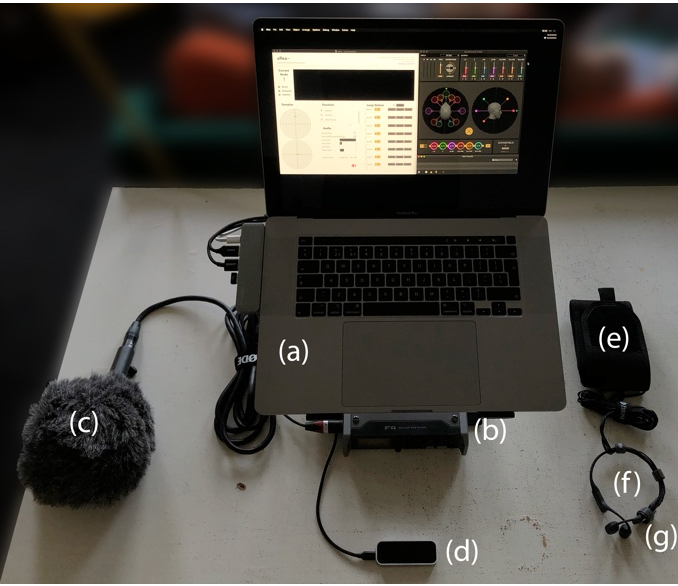
\includegraphics[height=5.5cm]{figures/05-area/areatechnical_hardware.png}}%
    
    \subcaptionbox*{}[.45\textwidth]{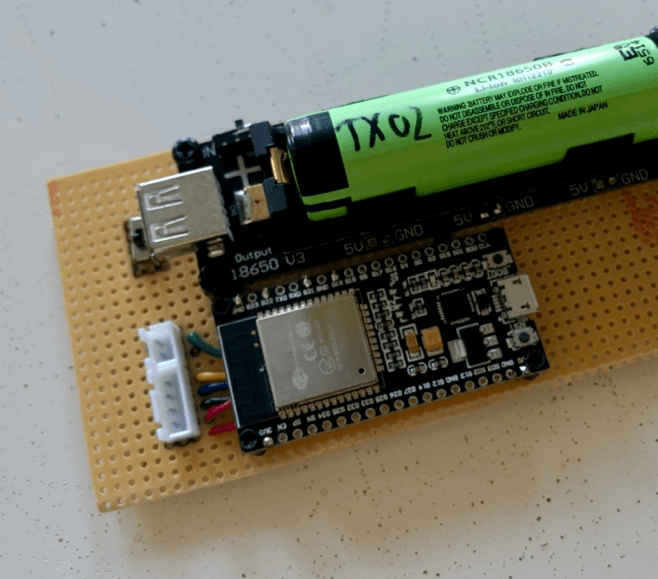
\includegraphics[height=5.5cm]{figures/05-area/areatechnical_pcb.png}}%
    \caption{\textit{area\textasciitilde{}} hardware and PCB}
    \label{fig: areatechnical}
\end{figure}

The on-desk hardware for the \textit{area\textasciitilde{}} system shown in Figure 2 includes (a) a laptop running the Max MSP \footnote{\url{https://cycling74.com/products/max}} patch, (b) a 4 channel input audio interface, (c) an Ambisonic microphone, and (d) a Leap Motion Controller.

The wearable hardware used for the \textit{area\textasciitilde{}} system comprises 2 sections: (e) a belt pouch containing a PCB-mounted ESP32 microcontroller \footnote{\url{https://www.espressif.com/en/products/socs/esp32/overview}} and 18650 battery (shown in \autoref{fig: areatechnical}), and (f) a pair of bone conduction headphones \footnote{\url{https://aftershokz.co.uk/products/aeropex}}, with (g) a mounted inertial measurement unit (IMU) for tracking head orientation. 

The IMU and ESP32 are connected via a detachable 1.5m heat shrunk cable that runs from the back of the bone conduction headphones, down the length of the user's back and into the belt-mounted transmitter pouch. With the integration of an Arduino library \footnote{\url{https://github.com/kriswiner/ESP32/}}, the IMU data is transmitted to the laptop via Bluetooth from the ESP32. Audio is transmitted to the headphones via Bluetooth from the Max MSP patch running on the laptop. 

The only hardware that needs to be accessible for the person composing with \textit{area\textasciitilde{}} is the Leap Motion Controller and the wearable hardware system. The laptop and audio interface are ideally hidden from view so as to minimise distraction. The microphone should be placed in a location that will provide them with access to sounds that they wish to compose with.

\subsection{Software Implementation}            \label{sec: area-system-software}

%*[ ]   fix figure
\begin{figure}
    \centering
    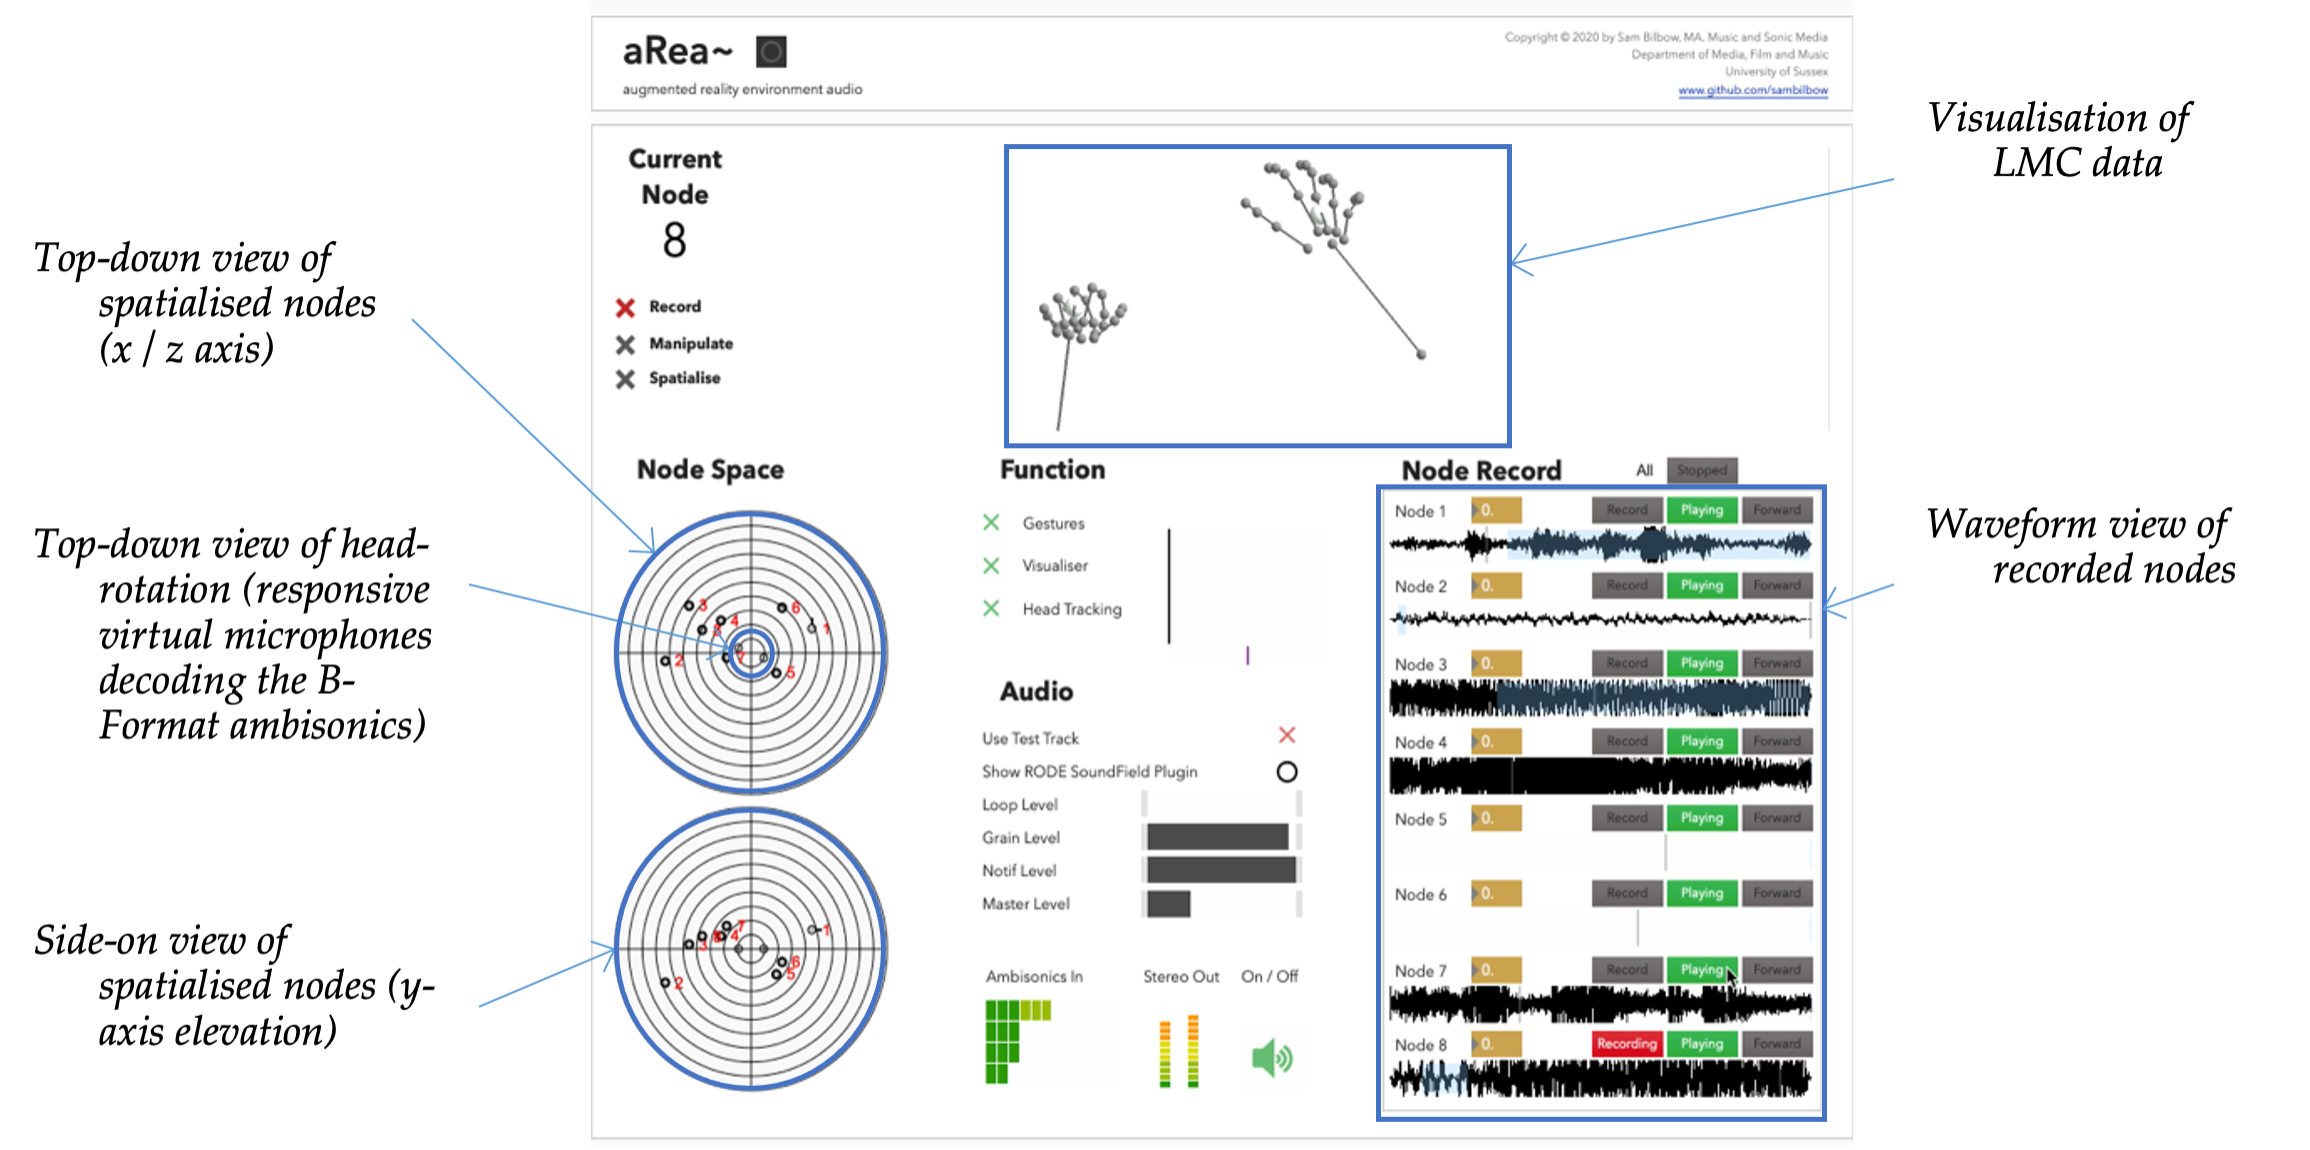
\includegraphics[width=\linewidth]{figures/05-area/areatechnical_max.png}
    \caption{\textit{area\textasciitilde{}} Max MSP patch}
    \label{fig: areatechnicalmax}
\end{figure}
The patch (\autoref{fig: areatechnicalmax}) uses the audio plugin \footnote{\url{https://www.rode.com/soundfieldplugin}} shown in \autoref{fig: areatechnicalrode} to encode the A-Format ambisonics microphone input into B-Format (a three-dimensional sound field), or what I will refer to as the \textit{ambisonic palette}. This \textit{ambisonic palette} is not heard by the composer; instead, they can sculpt from it, forming their own audible \textit{(B-Format) virtual audio environment} through hand gestures. I have defined these gestures in Max MSP with help from the IRCAM Leap Motion library \citeyearpar{ircam2014} \footnote{\url{https://github.com/JulesFrancoise/leapmotion-for-max}}, and they occur over three stages of interaction: \textit{\textbf{record, manipulate, spatialise}}. 

%*[ ]   fix figure
\begin{figure}
    \centering
    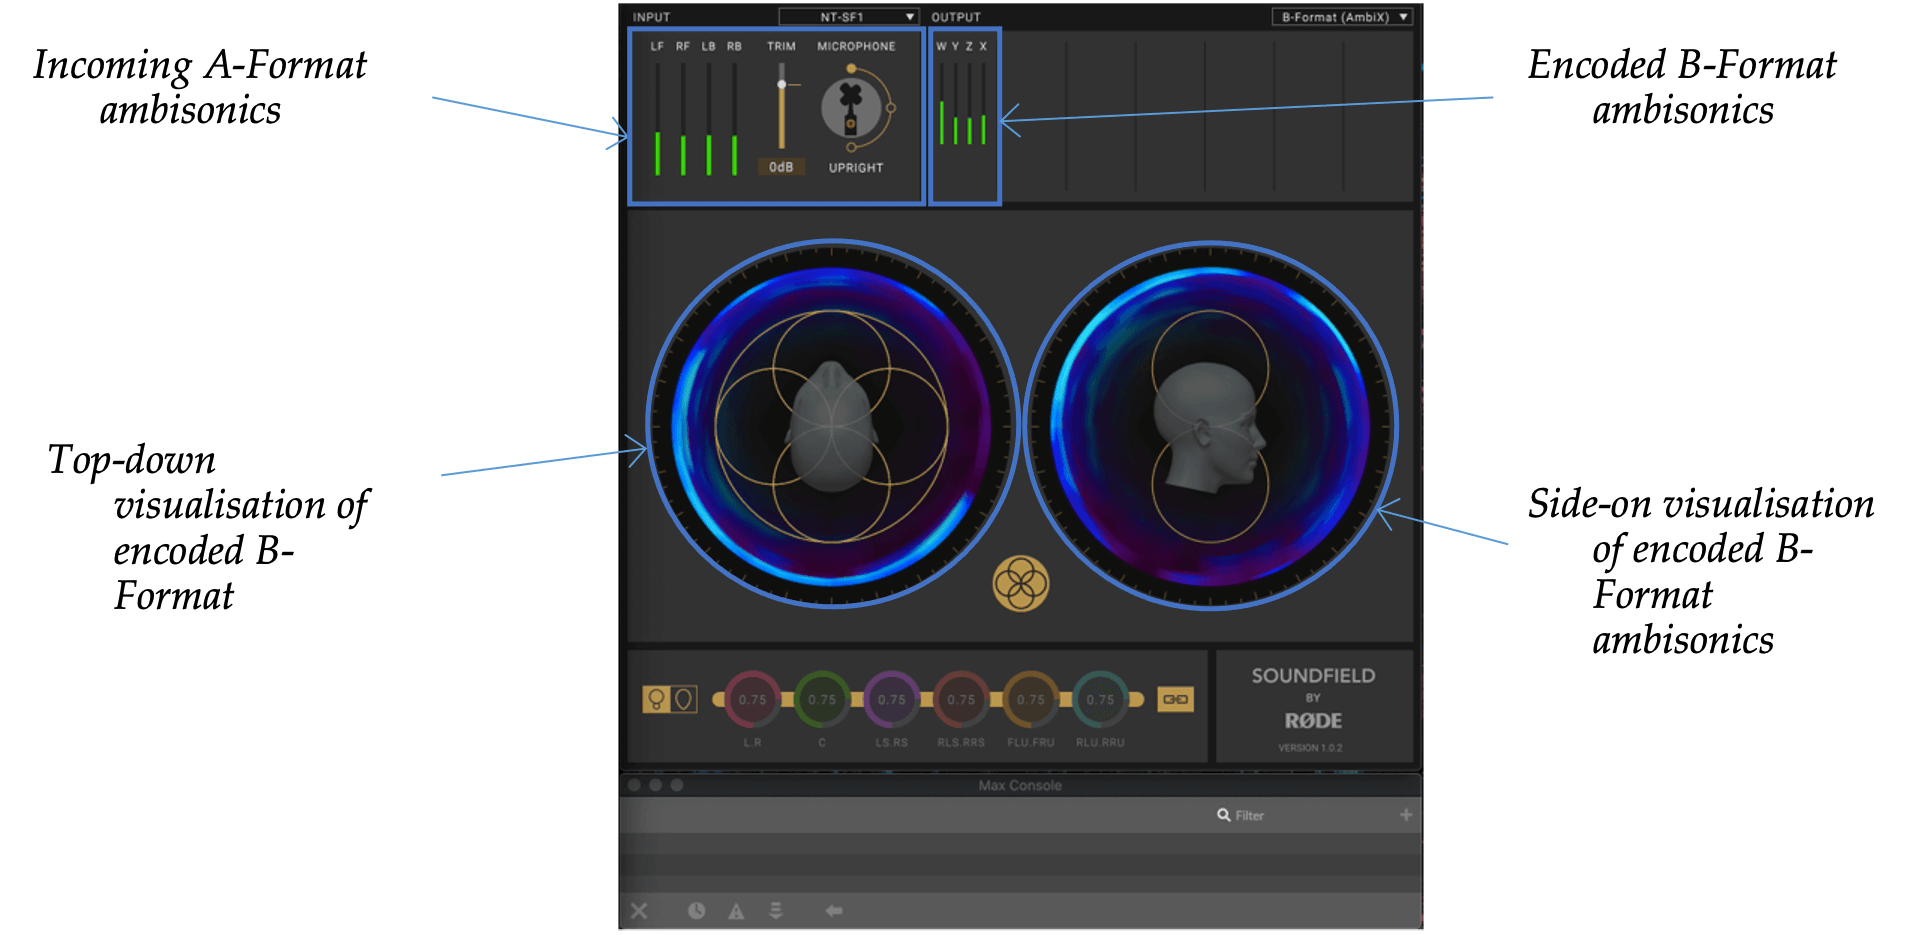
\includegraphics[width=\linewidth]{figures/05-area/areatechnical_rode.png}
    \caption{RØDE Soundfield Plugin}
    \label{fig: areatechnicalrode}
\end{figure}

\subsubsection{Record}                          \label{sec: area-system-software-record}
The \textbf{recording or ‘sampling’ stage} is initiated by making a left-hand grab above the LMC, the longer lasting the grab, the longer the portion of audio from the \textit{ambisonic palette} is sampled. The three-dimensional coordinates of the hand above the LMC correlates with the location of audio recorded (this is achieved by mapping the hand coordinates to a virtual microphone inside the \textit{ambisonic palette}), essentially allowing the composer to record sounds around their person in three dimensions. Upon letting go of the grab gesture, the sample plays on repeat (using the karma\textasciitilde{} Library \footnote{\url{https://cycling74.com/tools/karma-samplerlooper-external}}) through the bone conduction headphones, thus setting up the session’s \textit{virtual audio environment}.

\subsubsection{Manipulate}                      \label{sec: area-system-software-manip}
\textbf{The manipulation stage} is automatically initiated after the ending of the previous grab gesture and uses translational (x, y, z) and rotational (roll, pitch) values from both hands when above the LMC. There are two audio effects being manipulated, with parameters from these effects mapped in different ways to the translation and rotation of the composer's hands.
\begin{itemize}
    \item The first effect is a band-pass filter which accentuates certain audio frequencies of the sample. The frequency, strength, and gain of the filter is determined by the parameter mappings detailed in \autoref{fig: areaparams1}
    \item The second effect is a semi-random granular synthesiser. This selects and copies a section of the sample and deconstructs it into several hundred grains. The section of the sample granulised, and the individual grain duration is determined by the parameter mappings detailed in \autoref{fig: areaparams2} 
\end{itemize}
\begin{figure}
    \centering
    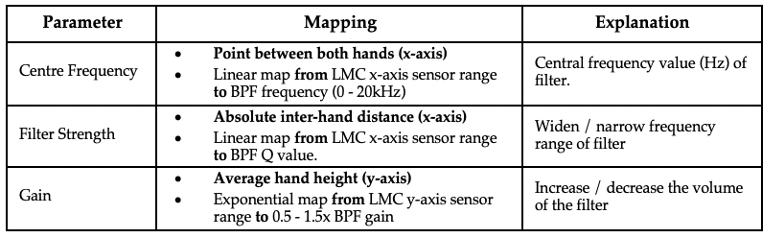
\includegraphics[width=0.8\linewidth]{figures/05-area/areatechnical_param1.png}
    \caption{Band-pass filter parameter mappings}
    \label{fig: areaparams1}
\end{figure}

\begin{figure}
    \centering
    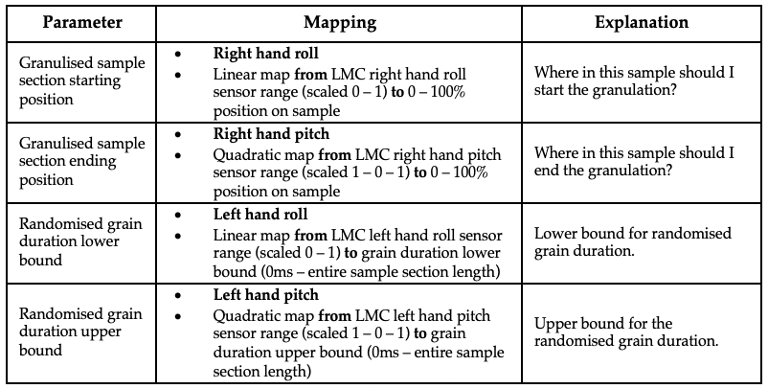
\includegraphics[width=0.8\linewidth]{figures/05-area/areatechnical_param2.png}
    \caption{Granular synthesiser parameter mappings}
    \label{fig: areaparams2}
\end{figure}
When the composer decides to end manipulating the sample, they can do so by performing a grab with both hands. Once this happens, the band-pass filter and granular synthesis parameters are frozen for that sample.

\subsubsection{Spatialise}                      \label{sec: area-system-software-spatialise}
\textbf{The spatialise stage} begins once the manipulation stage has ended. The three-dimensional space above the LMC is mapped to the \textit{virtual audio environment}, in which the composer is currently listening to the sample that they have recorded. The composer can use their right hand to move the sample around the \textit{virtual audio environment}. For an example of the effect this has, moving the hand between the two extremes of the x-axis (left to right) results in hearing the sample move from ear to ear. The spatialise stage is ended by grabbing with the right hand.

Once the spatialise stage has ended, the composer has the option to repeat the process 7 more times, allowing for the creation of a \textit{virtual audio environment} comprised of up to 8 spatialised audio samples, or what I refer to as \textit{nodes}. 

\subsubsection{Summary}                         \label{sec: area-system-software-summary}
The audio signal arriving in the two conduction pads in the headphones are the signals of two equidistantly spaced virtual microphones inside the \textit{B-Format virtual audio environment} that decode it into two channels, left and right. Further interaction comes from composer head movement which, at all times, is mapped to the revolution of these two virtual microphones around the central point of the \textit{virtual audio environment}. This means if there is a node playing to the left of the composer, rotating the head 90° anticlockwise results in the \textit{node} now sounding as if it is in front of the composer’s face. This is achieved via the ICST Ambisonics Library \citep{schacher2006} \footnote{\url{https://www.zhdk.ch/forschung/icst/software-downloads-5379/downloads-ambisonics-externals-for-maxmsp-5381}}and is elaborated on in the sections \autoref{sec: area-study-results-experiences} and \autoref{sec: area-discussion-aar}, but for now it is worth mentioning that it allows for immersion into a combined \textit{real and virtual audio environment}.

To summarise, the patch can be categorised into having two inputs: audio from the composer’s environment and hand gesture, and one output: \textit{the virtual audio environment}. In the background, this audio input is decoded into the \textit{ambisonic palette} (inaudible), which is acted on by the composer’s hands to form one audible output: the \textit{virtual audio environment}, which is comprised of up to 8 \textit{nodes}. Through the choice of sensory overlay (bone conduction) and integration of head tracking, this \textit{virtual audio environment} is experienced synchronously with the composers’ real, multisensory environment. 



% --------------------------------------------------------------------------- %
\section{Composing with \textit{area\textasciitilde{}}} \label{sec: area-study}
\subsection{Autobiographical Design}            \label{sec: area-study-abd}
Originally, the study was planned for late March and would involve several participatory interaction studies. However, due to the UK lockdown in response to the unfolding COVID-19 pandemic, this was postponed until later in the year. Instead, I investigated the system using an autobiographical design method, framing it as a hypothesis study to better understand relationships between virtual and real environments, in the hope of developing a practice-led method for creating and researching multisensory augmented reality experiences. 

Autobiographical design is defined as “design research drawing on extensive, genuine usage by those creating or building the system” \citep{neustaedter2012}. Neustaedter and Sengers define “genuine usage” here to mean that changes are “based on the true needs of the researchers, rather than them pretending to have needs expected of target users”.

Due to the lockdown, and therefore inability to conduct in-person user-tests, this research method was beneficial as I was spending large amounts of time with the system. Moreover, there are several suggested requirements of employing this research method that Neustaedter and Sengers highlight that are true of the \textit{area\textasciitilde{}} system:
\begin{itemize}
    \item The existence of a genuine usage of the system
    \item The system being already developed
    \item The ability for fast tinkering 
    \item Record-keeping of the design process
    \item Long-term usage of the system
\end{itemize}
Furthermore, as AR technology moves towards being a component of future general personal computing, there is a need for first-person research methods that take into consideration the effects of prolonged system usage as well as the arising relationship between participant and system \citep{desjardins2018}. Moreover, these methods have been found to be specifically relevant to wearable systems \citep{cecchinato2017}.

A disadvantage of using autobiographical design as a research method is its inability to establish generalisability (also the case with ethnography, case studies and participatory workshops), which is why I opted for participant studies in the evaluation of \textit{polaris\textasciitilde{}} in \autoref{sec: polaris}.

\subsection{Design} \label{sec: area-study-design}
The study was designed as a cycle, in order to promote fast tinkering, record-keeping, and long-term usage in line with autobiographical design guidelines. 
\begin{enumerate}
    \item Over three sessions, ideally during the same week, the system is used with a logbook at hand in order to facilitate record-keeping of hardware setup, \textit{node} manipulation and completed \textit{real and virtual audio environment} listening experience remarks.
    \item After each session, the notes are formalised into a database and categorised as "composer experience remarks” or “improvement remarks”.
    \item At the end of the week, the three sessions’ notes are summarised into a “check-in” document, where composer experience remarks are collated, and improvement remarks are further categorised into lists pertaining to the area of the system that needs improvement or change.
    \item Those changes are then made to the system and the cycle restarts.
\end{enumerate}

\subsection{Results}                            \label{sec: area-study-results}
\subsubsection{Hardware Location}               \label{sec: area-study-results-hwloc}
I have observed that an environment with a lower noise floor is desirable and have implemented a normaliser to deal with re-recording loud background / ambient noises during successive \textit{node} recording. I found myself basing the choice of microphone placement on what I wanted the \textit{virtual audio environment} to sound like. Since the system uses an ambisonic microphone, consideration of the spherical 360° field of the microphone would lead to a richer \textit{ambisonic palette} and subsequent \textit{virtual audio environment}.

Two sessions were based outdoors and involved natural sounds such as birds, trees and wind, as well as passing cars. One of the sessions was inside and took place at the same time my partner was on a Zoom call, and therefore the \textit{ambisonic palette} was invariably based on her speech and my movement and action inside the room. I want to look into placing the microphone inside bushes, trees, etc. rather than in open spaces to explore aesthetically the \textit{virtual audio environment} that arises from such placement. Furthermore, the relationship between \textit{real and virtual audio environment} would be quite different. Through their ears, the composer would be rooted in their position in the environment, but because of the inherent blend between hearing and bone conduction, they would simultaneously experience the sonic environment of the bush mediated by the Max MSP patch.

\subsubsection{Experiences}                     \label{sec: area-study-results-experiences}
The system takes considerable time to set up, especially when documenting with video, audio, and notes. This process could certainly be streamlined further. Overall, I was pleased with the sound quality; the microphone picks up the environment very clearly. However, I remarked that the manipulation stage could feature more interesting real-time auditory effects on the \textit{nodes}. The blending of \textit{real and virtual audio environment} is achieved well via the bone conduction headphones and there was a subconscious registration via the head-tracking that gave me the very real impression that there was a 3D environment of \textit{nodes} around my body.

The IMU on the bone conduction headphones sometimes provides erratic and erroneous data, leading to accidental revolutions of the \textit{virtual audio environment} around the head. Despite technical difficulties such as this, in one autobiographical design session, when I took the headphones off, I wrote that “I felt like I'd been disconnected from something” and that “my senses felt heightened before I took them off, not only to the \textit{virtual audio environment}, but now more sensitive to the audio content of my real environment.

If I managed to capture an infrequent environment sound, such as a particular bird call, or a sentence of spoken word, the fact that the patch is set up to loop the samples gave a certain permanence to that otherwise impermanent sound. On multiple occasions I could not tell if the sounds of birds I was hearing originated from a \textit{node} or from within a tree.

\subsubsection{Arising Interactions}            \label{sec: area-study-results-arisingints}
The maximum sample length is currently 28 seconds, but I have found myself mainly sticking to shorter loops, creating quite repetitive and rhythmic sequences. I remarked that grains from the synthesiser sounded like a permanent record of my gestures’ effect on the environment. I liked the playfulness of being able to record a sound from a certain location in my \textit{real audio environment} and place it in different location in my \textit{virtual audio environment}.

Despite the wearable hardware being wireless, hand interaction with the \textit{area\textasciitilde{}} system is inherently limited to being in range of the LMC (often placed on a table). I found myself wanting to be able to move around my environment whilst being able to record new nodes and hear existing nodes move relative to my body position.
\section{Evaluating \textit{area\textasciitilde{}}} \label{sec: area-discussion-aar}
Overall, the results from my autobiographical design method have shown that \textit{area\textasciitilde{}} is an effective tool for examining the combinatorial relationship between real and virtual environments. Despite the system’s hardware setup requiring some further work to allow for quicker start up and more accurate head tracking, it has provided me with novel aesthetic experience through:
\begin{itemize}
    \item The blending of \textit{real and virtual auditory environments} to create a third, augmented environment that was greater in experiential nature than the sum of its parts (not simply a combinatorial layering)
    \item The ability to spectromorphologically manipulate sounds in real-time in this third environment with the body
    \item The potential for creating believable illusions of real-world sound sources from these manipulated and spatialised virtual sounds.
\end{itemize}

The tables of parameter mappings shown in \autoref{sec: area-system-software-manip} may seem like a chaotic mess, however, time has been spent making these mappings intuitive. For example, the representation of volume to a vertical scale corresponds with findings that non-musicians are relatively competent at attributing the size of air-gestures to heightened musical dynamics \citep{godoy2006,caramiaux2010}. As for the band-pass filter’s horizontal pitch mappings, this is mainly based on the visual representation of frequencies on a horizontal scale often found in the user interface of such filters. Nevertheless, it is pertinent to mention that field of psycho-musicology research \citep{timmers2016} finds a correlation between pitch representation and horizontal space i.e. lower pitch to the left, higher pitch to the right. Although this is often attributed to the internalised representation of horizontal pitch on pianos by keyboard-playing musicians \citep{lidji2007,rusconi2006}, it has been found that this effect also propagates in non-musicians \citep{weis2016}. This is also found to be the case in the “Playing air-instruments” study carried out by Godøy, Haga, and Jensenius \citeyearpar{godoy2006}.

In contrast, interaction with the granular synthesiser is not made to be intuitive; instead, I have opted to hide or black-box the interaction through a mix of linear and quadratic mappings on each hand. This is in order to stir curiosity in the composer and induce play, as I found in \autoref{sec: area-study-results-arisingints}: “I remarked that grains from the synthesiser sounded like a record of my gestures’ effect on the environment”.

Indeed, whilst outlining the material epistemologies of digital music instruments (DMIs), \citep{magnusson2009} describes black-boxed DMIs as containing  “knowledge of its inventors, which means that the users of the instrument do not need to have a deep knowledge of its internal functions”, furthermore clarifying that there is a “continued oscillation between a mode of conceptual (system design) engagement with the instrument and [an] embodied (performative) relationship with it”. This ‘oscillation’ displays, in turn, an underlying synergy between DMI development and the autobiographical design process, perhaps due to the similarities in requirements of the processes outlined in \autoref{sec: area-study-abd}. This synergy has led to the use of ABD in the development of many DMIs and interactive music systems \citep{kiefer2020,martin2017,turchet2018,unander-scharin2014}.

\begin{figure}
    \centering
    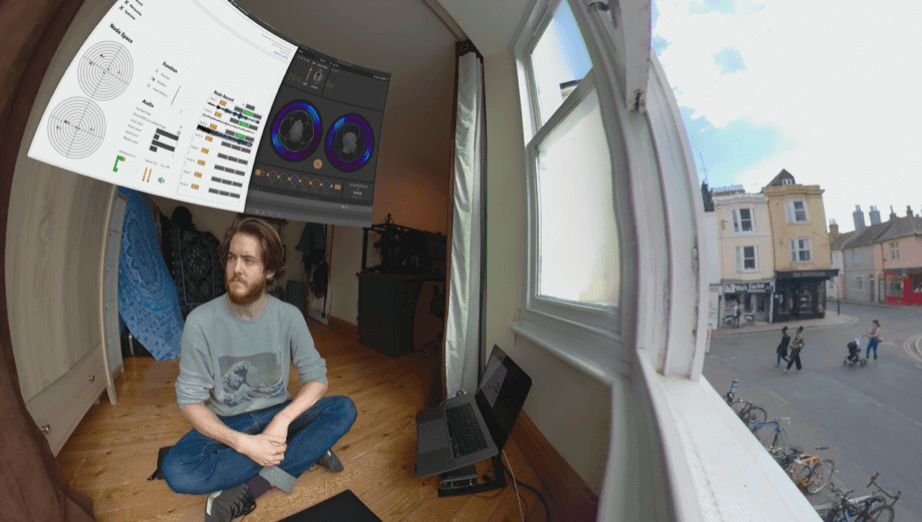
\includegraphics{figures/05-area/areafuturedoc.png}
    \caption{\textit{area\textasciitilde{}} 360° video and ambisonic documentation \rurl{youtu.be/SPd-f2EXuIQ}}
    \label{fig: areafuturedoc}
\end{figure}
As a system for creating computational sound ARt in the form of in-situ AAR experiences, \textit{area\textasciitilde{}}’s artistic output is firstly a real-time compositional experience. In order to document these experiences of the system however, I have included the automated recording and saving of both the \textit{ambisonic palette} (the ambisonic recording of the real audio environment), and the users \textit{virtual audio environment} as separate B-Format .wav files in the project directory. These separate B-Format .wav files could be merged and decoded from B-Format to any number of speakers for a multi-channel installation of field recordings or manipulations of environments made with \textit{area\textasciitilde{}}. This also leaves open the potential for \textit{area\textasciitilde{}} to be used as a compositional tool for interactive soundscape composition.

I also chose to merge and decode a set of these recordings to binaural stereo format, and have time-synced this recording with a 360° video and a screen recording of the patch that was taken during the system’s use. This allows my composition of the \textit{virtual audio environment} to be experienced second-hand with headphones. Dragging the screen in different directions with mouse/touchscreen emulates hearing the difference in environment if I moved my head in those directions. Optionally, an inexpensive smartphone VR headset (£5 - £15) can be used to heighten the interactivity of the experience. A screenshot of the 360° video \citep{bilbow2020} is shown in \autoref{fig: areafuturedoc}. The potential for users’ experiments with \textit{area\textasciitilde{}} to be captured and re-experienced interactively could have interesting applications, effectively allowing users to explore each others’ lived aural experience of the system.
% --------------------------------------------------------------------------- %



%The  novel experiences that emerged from the results of the study into the uses of AR as a medium for computational art have encouraged me to devise a practice-led method for researching multisensory AR (MSAR). It begins with the ideation of an MSAR Experience (which describes a possible human-to-sense interaction). These are classed as Snippets, Scenes, and Spaces depending on the number of senses engaged, sensory intensity, and interaction size. The hardware and software that enable the experience are classed as MSAR Instruments and MSAR Environments respectively. Instruments are categorised into Wearable, Tangible and Situated Instruments. This taxonomy will eventually aid not only in the creation, but in the evaluation of future MSAR Experiences. 